%%%============================================================================
%
%   Pandoc template to convert to latex using emulateapj.
%   
%
%   Usage:
%   ------
%
%   pandoc --template=[/Path/To/File/]pandoc-apj.latex
%
%
%
%   Caveats (mostly limitations in pandoc):
%   ---------------------------------------
%
%   + Doesn't do figure* and table* environments, these must be tweaked 
%     manually from standard figure and table environments or inserted as raw
%     LaTeX rather than Markdown figure invironments.
%     UPDATE: This can be accomplished by using Scholdoc rather than Pandoc.
%   + Same goes for equations: pandoc (at the time of writing) only does
%     displaymath, equations must be declared in raw LaTeX
%   + Graphics are not scaled, because the autoscale function provided in the
%     template is using the raw TeX \def function, which is not supported in
%     ApJ. UPDATE: This has been fixed in Pandoc, and Scholdoc even better.
%     Use Scholdoc! 
%
%   Copyright 2014-2016 T. E. Rivera-Thorsen.
%
%%%============================================================================
\documentclass[twocolumn]{aastex61}
% \usepackage{lmodern}
% \usepackage{dcolumn}
\usepackage{amssymb,amsmath}
\usepackage[T1]{fontenc}
\usepackage[utf8x]{inputenc}
% \usepackage{natbib}
\bibliographystyle{aasjournal}
\usepackage{listings}
\usepackage{graphicx}
%\ifxetex
%  \usepackage[setpagesize=false, % page size defined by xetex
%              unicode=false, % unicode breaks when used with xetex
%              xetex]{hyperref}
%\else
%\usepackage[unicode=true]{hyperref}
%\fi
\hypersetup{breaklinks=true,
           bookmarks=true,
           pdfauthor={},
           pdftitle={Neutral ISM, Lyman-Alpha and Lyman-continuum in nearby starburst Haro 11},
           colorlinks=true,
           citecolor=blue,
           urlcolor=blue,
           linkcolor=magenta,
           pdfborder={0 0 0}}
\urlstyle{same}  % don't use monospace font for urls
% \setlength{\parindent}{0pt}
% \setlength{\parskip}{6pt plus 2pt minus 1pt}
% \setlength{\emergencystretch}{3em}  % prevent overfull lines
% \setcounter{secnumdepth}{5}

\shorttitle{Neutral ISM, Ly-Alpha and LyC in Haro 11}

\shortauthors{T. E. Rivera-Thorsen et al.}



%% Command to document which AAS Journal the manuscript was submitted to.
%% Adds "Submitted to " the arguement.





% % \date{\today}
% 
\usepackage[caption=false]{subfig}

%%%-----------------------------------------------------------------------
%      Macros
%%%-----------------------------------------------------------------------
\begin{document}


\title{Neutral ISM, Lyman-Alpha and Lyman-continuum in nearby starburst Haro 11}

\title{Neutral ISM, Lyman-Alpha and Lyman-continuum in nearby starburst Haro 11
		                    \footnote{Based on observations with HST-COS, program GO 13017, PI Heckman}
	            }
%
\correspondingauthor{T. Emil Rivera-Thorsen}
\email{trive@astro.su.se}

\author{T. Emil Rivera-Thorsen}
\affil{Department of Astronomy, Stockholm University, AlbaNova University
Centre, SE-106 91 Stockholm, Sweden}
\affil{Oscar Klein Centre for Cosmoparticle Physics, Stockholm, Sweden}
\author{Göran Östlin}
\affil{Department of Astronomy, Stockholm University, AlbaNova University
Centre, SE-106 91 Stockholm, Sweden}
\affil{Oscar Klein Centre for Cosmoparticle Physics, Stockholm, Sweden}
\author{Matthew Hayes}
\affil{Department of Astronomy, Stockholm University, AlbaNova University
Centre, SE-106 91 Stockholm, Sweden}
\affil{Oscar Klein Centre for Cosmoparticle Physics, Stockholm, Sweden}
\author{Johannes Puschnig}
\affil{Department of Astronomy, Stockholm University, AlbaNova University
Centre, SE-106 91 Stockholm, Sweden}
\affil{Oscar Klein Centre for Cosmoparticle Physics, Stockholm, Sweden}


\begin{abstract}
Star forming galaxies are believed to be a major source of ionizing
radiation responsible for reionizing the early Universe. Direct
observations of escaping ionizing radiation have however been few and
with escape fractions far below what would be necessary to account for
the ionization history of the Universe. In the local Universe, only a
few handfuls of emitters have been observed with typical escape
fractions of a few percent. It seems the mechanisms regulating this
escape need to be strongly evolving with redshift, if galaxies are to be
held responsible for reionization. Gas mass, star formation feedback and
thus star formation activity are among the main suspect parameters,
known to both regulate neutral gas coverage and evolve with cosmic time.
In this paper, we present a reanalysis of far-UV HST-COS spectra of the
first detected Lyman-continuum leaker in the local Universe, Haro 11, in
which we examine the connections between Lyman-continuum leakage and
Lyman-$\alpha$ line shape and feedback-influenced neutral ISM properties
like kinematics, geometry and column density. We discuss the two
extremes of an optically thin, density bounded ISM and a riddled,
optically thick, ionization bounded ISM and how Haro 11 fits into the
theoretical predictions made from these models. We find that the most
likely ISM model for Haro 11 knot C is one of clumpy neutral medium
embedded in a highly ionized inter-clump medium with a combined covering
fraction of unity and a residual neutral gas column density in the
ionized medium of
$5 \times 10^{13} \leq N_{\rm HI} \leq 4 \times 10^{15}$; high enough to
be optically thick to Lyman-$\alpha$, but low enough to be at least
partly transparent to Lyman-continuum and undetected in Si\textsc{ii}.
\end{abstract}

\section{Introduction and
Observations}\label{introduction-and-observations}

Even though star forming galaxies are believed to give rise to the
majority of radiation reionizing the Universe at early times, it remains
unknown which physical conditions can facilitate the escape of the
necessary amounts of radiation from these galaxies, which contain large
amounts of neutral gas opaque to this radiation at higher column
densities. Searches for leaking galaxies at redshifts $z \gtrsim 1$ have
yielded few detections
\citep[e.g.][]{Iwata2009, Vanzella2010, Vanzella2012, Nestor2013, Cowie2009, Siana2010},
at escape fractions well below the $\sim 20\%$ needed to account for
cosmic reionization \citep{Bouwens2011, Robertson2013}. A population of
lower mass and lower luminosity, star forming galaxies are expected to
contribute to reionization, too, but high star formation is usually
coincident with higher neutral gas mass, which would cause a higher
probability of blocking the ionizing photons
\citep[e.g.][]{Erb2016, Robertson2013}. In the local Universe, only 9
leakers have been detected so far
\citetext{\citealp{Bergvall2006}; \citealp{Leitet2011}; \citealp{Leitet2013}; \citealp{Borthakur2014}; \citealp[Izotov2016Nat;][]{Izotov2016MNRAS}; \citealp{Leitherer2016}},
at escape fractions ranging typically between 1-8\%, with one as high as
$f_{\mathrm{esc}} \approx 13\%$ \citep{Izotov2016MNRAS}.

Models of ISM surrounding a central source and allowing escape of Lyman
continuum (LyC), span the range of two extremes: In one regime, the
surrounding gas is optically thin, highly ionized and density-bounded
\citep[see e.g.][]{Jaskot2013}, allowing unblocked escape for at least a
fraction of ionizing photons. In the other regime, the central source is
surrounded by an optically thick, ionization bounded medium with the
neutral medium surrounding the central Strömgren sphere not completely
covering all lines of sight to the background source. This is what is
called the \emph{picket fence model} by \citet{Heckman2011}, or the
\emph{riddled ionization bounded medium} by \citet{Verhamme2015}. The
latter paper presents modeling of the imprints of these two extreme
scenarios on the observed spectral signature of Lyman-$\alpha$ emission
lines, and suggest how these can help point to candidate LyC leakers.
The authors compare their theoretical predictions to sample of
Lyman-$\alpha$ profiles, including a section of the spectrum treated in
this work.

The present HST-COS observation is part of the sample in
\citet{Heckman2015} and \citet{Alexandroff2015}, in which details about
observation and data reduction are described in depth; we point the
reader there for further information about these. The Ly$\alpha$ profile
in this spectrum is discussed in \citet{JaskotOey}.

In (Rivera-Thorsen et al., submitted to \apj), we analyzed optical and
NUV nebular emission lines in slit spectra from ESO VLT/X-Shooter
\citep[see also][]{Guseva2012}. We find from kinematics modelling that
both knot B and knot C are associated to a component blueshifted by
$\sim 50 - 100$ km s\textsuperscript{-1} wrt. the mean nebular velocity.
This component reaches as far as $\sim 200$ pc. SE of knot B, and
$\sim 1.5$ kpc S of the midpoint between the two knots. Given the dense
cloud coverage of knot B and the strong star formation activity in both
knots, we conclude that this component is not only approaching but also
found in front of the starburst regions and thus along the LOS to knot
C.

Recently, the galaxy has been observed in 21 cm H\textsc{i} emission
with the 100 m. Robert C. Byrd Green Bank Telescope
\citep{Pardy2016arXiv}. The authors find that Haro 11 has a low gas mass
and a very low neutral gas to stellar mass fraction, and that it
contains around twice as much ionized as neutral Hydrogen.
Interestingly, the authors also find that the bulk of the neutral gas is
redshifted wrt. the systemic velocity defined from nebular emission from
the H\textsc{ii} regions surrounding the main starbursts, signifying
that the majority of the neutral gas reserves are detached from the star
formation activity, possibly a tidal arm being flung outwards as a part
of the ongoing merger event.

In this paper, we re-analyze the HST-COS spectrum of Haro 11 C acquired
as part of HST program GO 13017, PI Timothy Heckman. It was first
published in \citet{Alexandroff2015} as part of a sample of 22 Lyman
Break Analog (LBA) galaxies analyzed individually and as a stack. These
authors mainly focus on three indirect indicators of LyC leakage
\citep{Overzier2009, Heckman2011}: Residual flux in the trough of
saturated ISM absorption lines, blueshifted emission in Lyman-$\alpha$,
and weak optical {[}\ion{S}{2}{]} emission lines.

\begin{figure}
\centering
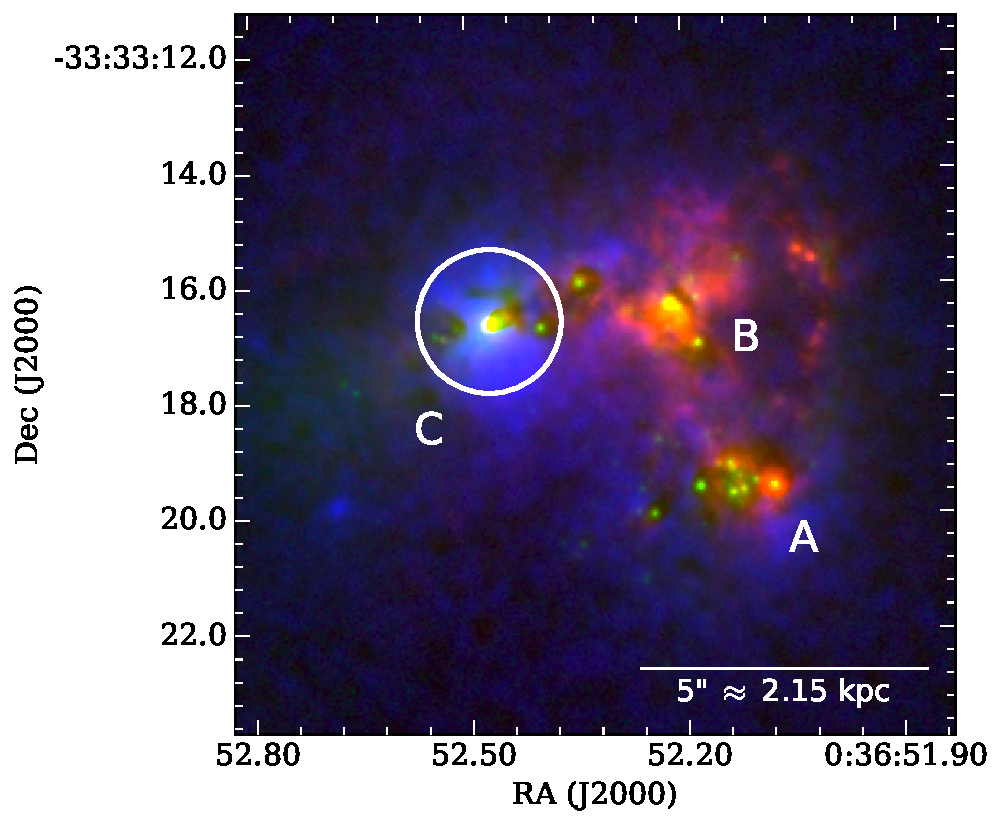
\includegraphics[width=3.500in]{../Figs/Haroslit.pdf}
\caption{Approximate position of the COS aperture, shown on HST imaging
data of \citet{Hayes2009}; \citet{Ostlin2009}, encoding UV continuum in
green, H$\alpha$ in red, and continuum subtracted Lyman $\alpha$ in
blue. N is up, E is to the left.}\label{fig:apert}
\end{figure}

We measure a number of kinematic parameters for both the neutral (LIS)
and high-ionized (HIS) phase, and apply the apparent optical depth
method \citep{Savage1991, Pettini2002, Quider2009, Jones2013}, with the
implementation being as described in \citet{RiveraThorsen2015} (RT15),
to infer geometric properties of the neutral medium and constrain the
column density of neutral hydrogen covering the background source under
the assumption that the LyC photons detected from this galaxy do indeed
escape from knot C.

\begin{figure*}
\centering
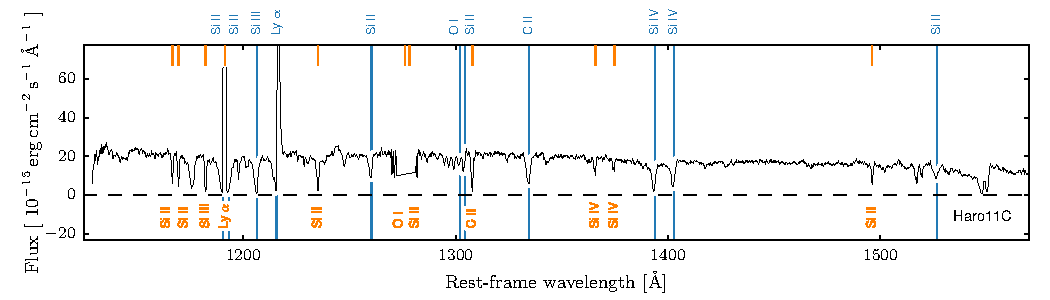
\includegraphics[]{../Figs/FullSpec.pdf}
\caption{Overview of the relevant regions of the COS spectrum of Haro 11
C, shown in rest frame wavelengths of the object. Some key spectral
lines are marked; Milky Way features in orange, features of Haro 11 in
blue.}\label{fig:fullspec}
\end{figure*}

Fig.~\ref{fig:fullspec} gives an overview of the COS spectrum of Haro 11
C treated in this work. Some important features are marked in blue
(internal to Haro 11) or orange (Milky Way features).

\subsection{Effective resolution}\label{effective-resolution}

For a point source, the resolution of the Cosmic Origins Spectrograph is
$R=20,000$, which corresponds to six pixels of the extracted spectrum
per resolution element. We have therefore binned the data by a factor of
6 to minimize noise while not losing information. The resolution,
however, is generally lower than this for extended sources; for a
uniformly filled aperture, it is as low as $R\approx2,000$. For more
morphologically complex sources, the effective resolution depends on the
exact shape and angular size of the target.

To estimate the effective resolution for this target, we proceeded as
follows. We used archival imaging data of Haro 11 in the UV-continuum
from \citet{Ostlin2009}; \citet{Hayes2009}; since the absorption lines
treated here have resolution determined by the properties of their
surrounding continuum. We the extracted a circular image at the same
position and radius as the COS aperture, which was rotated to match the
orientation of the COS as given in the spectrum headers. We then
modelled vignetting in the COS aperture by multiplying each pixel in the
circular UV-continuum image with an interpolation of the values given in
the throughput grid in Fig. 7 in \citet{CosImaging}. Finally, the
aperture cutouts were collapsed along the cross-dispersion direction,
and the FWHM of the flux distribution along the dispersion direction is
reported as the effective seeing of this observation. This is converted
from arc seconds to COS resolution elements by the factor 0.171
arcsec/resel reported in the COS instrument handbook \citep{CosHandbook}

\begin{figure}
\centering
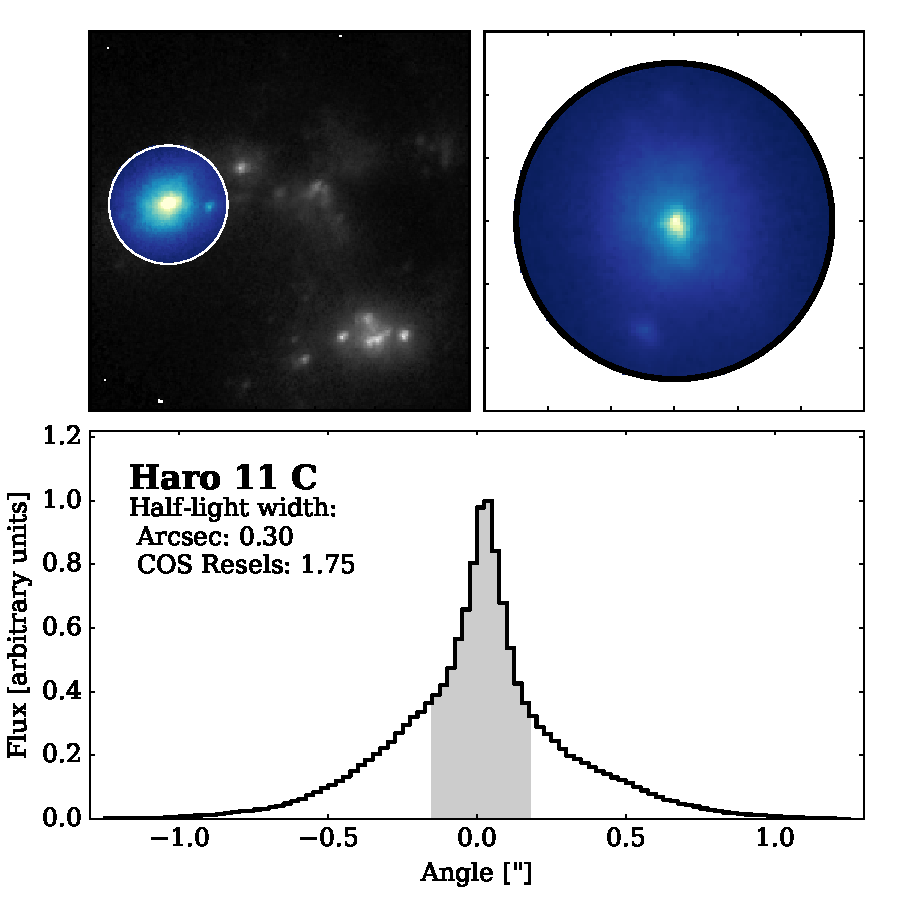
\includegraphics[width=1.000\hsize]{../Figs/EffResol.pdf}
\caption{Effective resolution estimate. \textbf{Upper left}: Haro 11 in
UV-continuum, data from \citet{Ostlin2009}; \citet{Hayes2009}. Data is
shown on a square root scale and cut levels set for best detail. Inset
in blue tinting is the COS aperture covering the region surrounding knot
B in the terminology of \citet{Vader1993}. N is up, E is left.
\textbf{Upper right}: The extracted, throughput-corrected in-aperture
image, rotated so horizontal corresponds to the dispersion direction of
the spectrograph. \textbf{Lower panel}: The collapsed flux profile in
the aperture, with the shaded region showing the width of the effective
resolution element, which is also given in arc seconds and resolution
elements/bins.}\label{fig:resol}
\end{figure}

The procedure is illustrated in Fig.~\ref{fig:resol}. Here, the upper
left panel shows Haro 11 in UV-continuum using HST imaging data from
\citet{Ostlin2009}; \citet{Hayes2009}, with the COS aperture coverage
from this observation overlaid in blue tinting. The upper right panel
shows the galaxy as the COS saw it, with the region covered by the
aperture cut out, rotated and vignetting-corrected as described above.
Finally, the lower panel shows the flux profile in the aperture,
collapsed along the cross dispersion direction. The FWHM of this
distribution has been adopted as the effective resolution for this
observation. We find $R_{\text{eff}} = 0.3 \arcsec = 1.75$ resolution
elements, which at the wavelength of observed Ly$\alpha$ corresponds to
31 km s⁻¹.

\section{Analysis}\label{analysis}

\subsection{Individual lines}\label{individual-lines}

Figure~\ref{fig:SingleLines} shows the individual profiles of the
transitions included in our analysis; the upper panel shows transitions
of \ion{Si}{2}, lower panel of \ion{Si}{4}. It is plainly visible that
the ionization fraction is high, with the \ion{Si}{4} curves being
considerably deeper than the low-ionized lines. Looking at the upper
panel, \ion{Si}{2} $\lambda \lambda 1304, 1526$ are somewhat shallower
than \ion{Si}{2} $\lambda 1260$. The former two lines have comparable
oscillator strengths, both about a factor of 10 lower than that of
$\lambda 1260$. It is thus clear that we do not find ourselves in the
optically thin regime, in which the latter line should be
correspondingly around 10 times stronger; on the other hand, it is
possible that the two weak lines are not completely saturated. In the
lower panel, the two \ion{Si}{4} lines have oscillator strengths within
a factor of 2 of each other. They are thus at first glance consistent
with a medium that is not completely opaque, but not with an optically
thin one, and within uncertainties consistent with the optically thick.
The stronger absorption in \ion{Si}{4} reveals a high level of
ionization of the medium covering the central cluster.

\begin{figure}
\centering
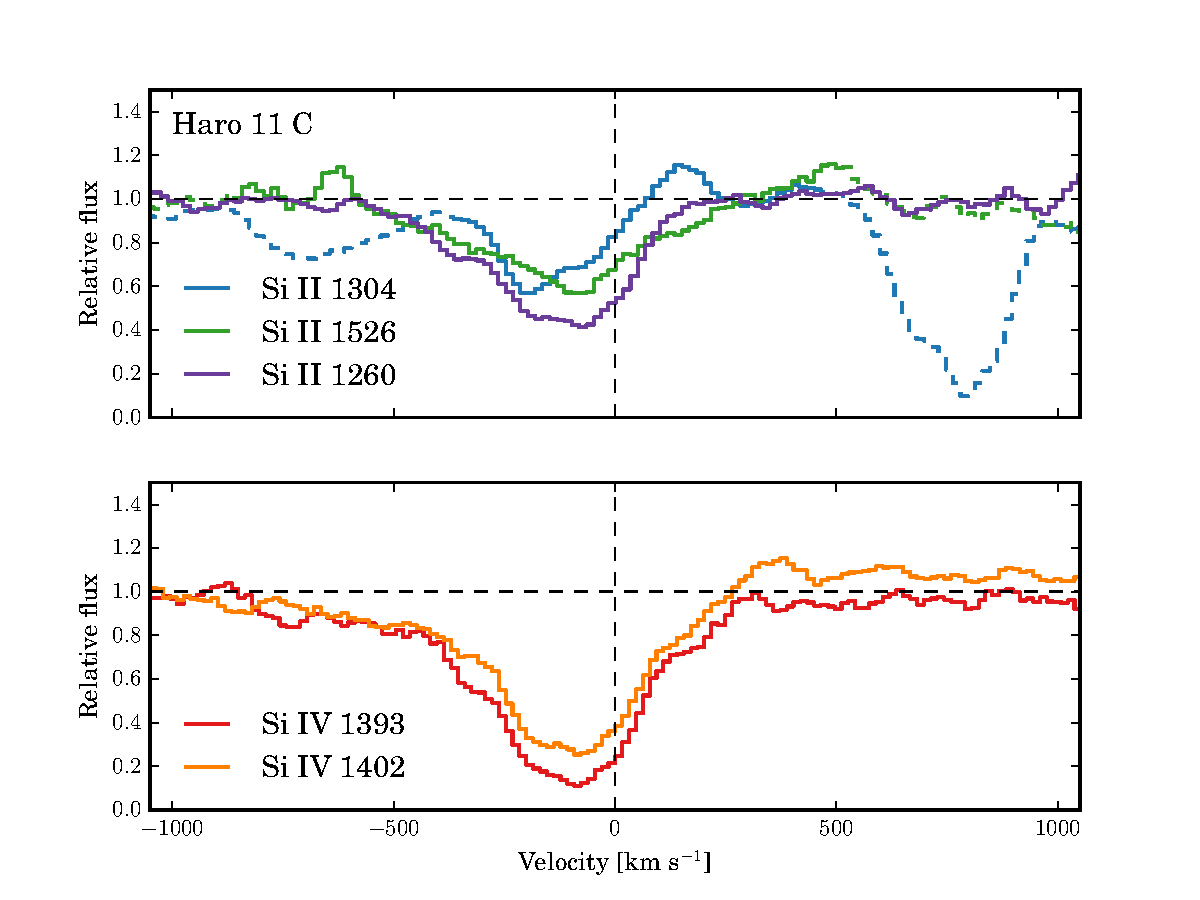
\includegraphics[width=3.500in]{../Figs/HISLISProfiles.pdf}
\caption{The \ion{Si}{2} and other LIS (\textbf{upper}) and \ion{Si}{4}
(\textbf{lower}) profiles included in this study. Dashes denote data
points masked out due to foreground contamination. Note the
high-velocity component in both \ion{Si}{4} lines, extending out to
$\sim 850$ km s⁻¹.}\label{fig:SingleLines}
\end{figure}

\floattable\

\begin{deluxetable}{lC} 
  \tablecaption{Measured properties}
  \tablehead{\colhead{Quantity} & \colhead{Haro 11 C} }
  %\colnumbers\
  \startdata
  $z$ \tablenotemark{a}   & 0.02043 \pm 0.00002  \\
  $z_v$ [km s⁻¹]  \tablenotemark{a} & 6126 \pm 7           \\
    $\Delta v^{\rm LIS}$            & 596 \pm 78           \\
    $v_{\mathrm{int}}^{\rm LIS}$    & -130 \pm 22          \\
    $v_{95\%}^{\rm LIS}$            & -421 \pm 64          \\
    $v_{\rm peak}^{\rm Ly\alpha}$    & 158 \pm 0.8         \\
    $\log_{10}(N_{\mathrm{Si II}})^{v = 0}$  &  12.1 \pm  0.2 \\
  \enddata\
  \tablenotetext{a}{From \citet{Sandberg2013}}
\end{deluxetable}


\subsection{$N_{\rm Si}$ and $f_C$}\label{sec:aod}

Following the method described in RT15, we have performed fits for
column density and covering factor in each velocity bin, for both the
high- and low-ionization state. Here we shall briefly summarize the
method, but refer to RT15 and references therein for a detailed
explanation.

In any given velocity bin, the line intensity in terms of the continuum
intensity is given as
%
\begin{equation}
\label{eq:II0}
\frac{I}{I_0} = 1 - f_C (1 - e^{-\tau}),
\end{equation}
%
 with the optical depth $\tau$ given as:
%
\begin{equation}
\label{eq:tau}
\tau = f\lambda \frac{\pi e^2}{m_e c} N 
       = f\lambda \frac{N}{3.768 \times 10^{14}}
\end{equation}
%
 Here, $f$ is the oscillator strength of a given transition, $\lambda$
is its rest frame wavelength in Å, $N = N(v)$ is the column density of
the relevant ion \emph{within the given velocity bin}, and $f_{C}$ is
the covering fraction of neutral gas \emph{moving at the given
velocity}. When multiple absorption lines are present which arise from
the same ground state; the population of this state is the same for all
transitions, and their relative strengths are governed simply by their
oscillator strengths, and with two or more such transitions, $f_{C}$ and
$N$ can be inferred from knowledge of $f \lambda$ and measured values of
$I/I_0$.

\begin{figure}
\centering
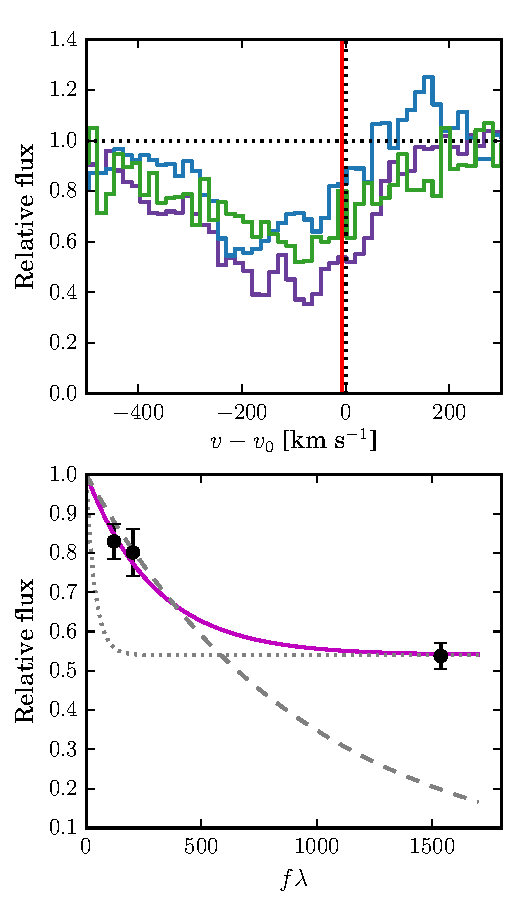
\includegraphics[width=0.800\hsize]{../Figs/AOD-details-example.pdf}
\caption{Illustration of the AOD computations. \textbf{Upper panel}: the
three \ion{Si}{2} lines in this analysis shown together, with the
zero-velocity bin marked with a vertical red line. \textbf{Lower panel}:
From this bin, the three measured relative intensities are plotted
against $f\lambda$ as black dots, with vertical error bars showing the
error spectrum from the COS pipeline. Also shown is the best-fit
function $I/I0 (f \lambda)$ as defined above. Also shown for
illustration are the two extreme examples of a very high column density
and unchanged covering fraction, and of a very high covering fraction
but significantly lower column density.}\label{fig:AOD}
\end{figure}

The method is illustrated in Fig.~\ref{fig:AOD}: In the upper panel is
shown the line profiles of the three \ion{Si}{2} transitions included in
the analysis. The red vertical line marks the zero-velocity bin. From
this bin, the three relative fluxes are plotted in the lower frame
against their wavelength scaled oscillator strengths $f\lambda$ on the
$x$ axis. In magenta is shown the best fit of the function
$I/I_0 (f\lambda)$ described above. Also shown are two examples of
different parametrizations of this function, to show how the two
parameters influence its shape. One, in dotted gray, shows what happens
to the best-fit function when $N$ is raised strongly, while $f_C$ is
kept unchanged, while the other in gray dashes shows the curve for a
$f_C \approx 1$ and $N$ is $~0.5$ dex below the best-fit value. This is
of interest to the discussion of radiative transfer effects below in
sect.~\ref{sec:rt}.

The resulting values of $N_{\text{Si\textsc{ii}}}$ and $f_C$ are shown
in fig.~\ref{fig:WithColDens}. The upper panels show the pseudo-reduced
$\chi^2$ as defined in RT15 ( $=\chi^2 / (\mathrm{DOF} + 1)$) for each
bin, middle panels show the inferred column density in each bin, with
surrounding shaded columns showing the confidence intervals. In the
lower panels, the mean LIS line profile is shown in black with gray
shaded uncertainty intervals. On these are overlaid the best-fit values
of $f_C$ as colored dots, with surrounding shaded bars showing the
confidence intervals. We again caution that $f_C$ is the covering
fraction of neutral gas \emph{within the given velocity bin}, and hence
only provides a lower limit for the total, geometric neutral gas
covering fraction, since gas at different velocities generally does not
occupy the same projected area.

\begin{figure*}
\centering
\subfloat[LIS\label{coldenLIS}]{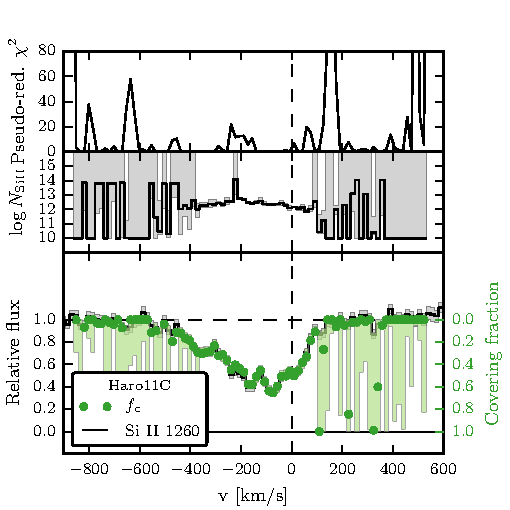
\includegraphics[width=0.400\hsize]{../Figs/Fc_haro11c_LIS.pdf}}
\subfloat[\ion{Si}{4}\label{coldenHIS}]{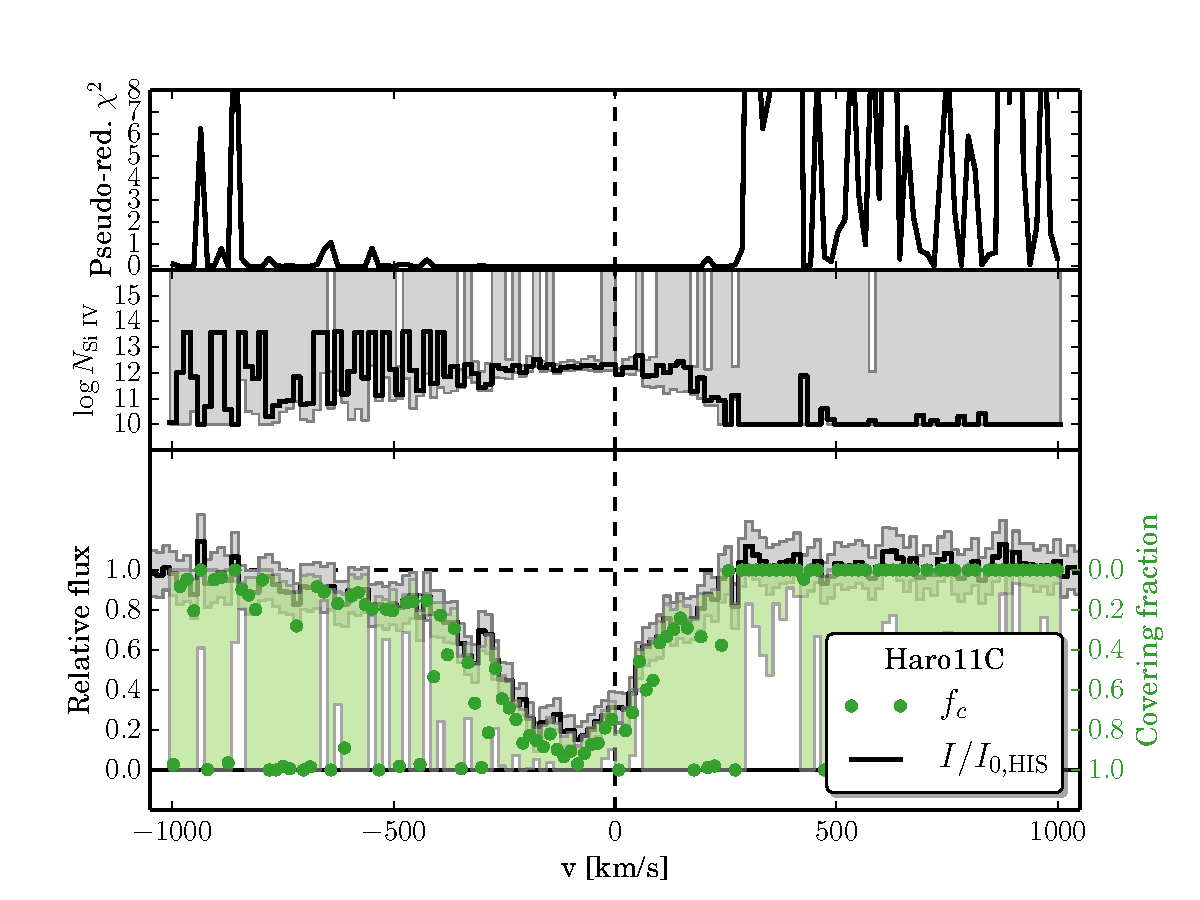
\includegraphics[width=0.400\hsize]{../Figs/Fc_haro11c-SiIV.pdf}}
\caption{\textbf{Upper panels}: Pseudo-reduced $\chi^2$ as described in
RT15. \textbf{Middle panels}: Best-fit ion column density with
confidence intervals in shaded gray. \textbf{Lower panels}: \ion{Si}{2}
1260 / mean\ion{Si}{4} profile shown as black steps, with inferred $f_C$
shown with yellow dots. Lighter shaded columns show confidence intervals
for both.}\label{fig:WithColDens}
\end{figure*}

\section{Discussion and conclusions}\label{discussion-and-conclusions}

\subsection{Lyman-$\alpha$ and ISM absorption
profiles}\label{sec:LISLya}

In fig.~\ref{fig:HisLisLya}, we show the neutral and ionized absorption
profile as in fig.~\ref{fig:WithColDens} together with the profile of
Ly$\alpha$ on a common velocity scale.

\begin{figure}
\centering
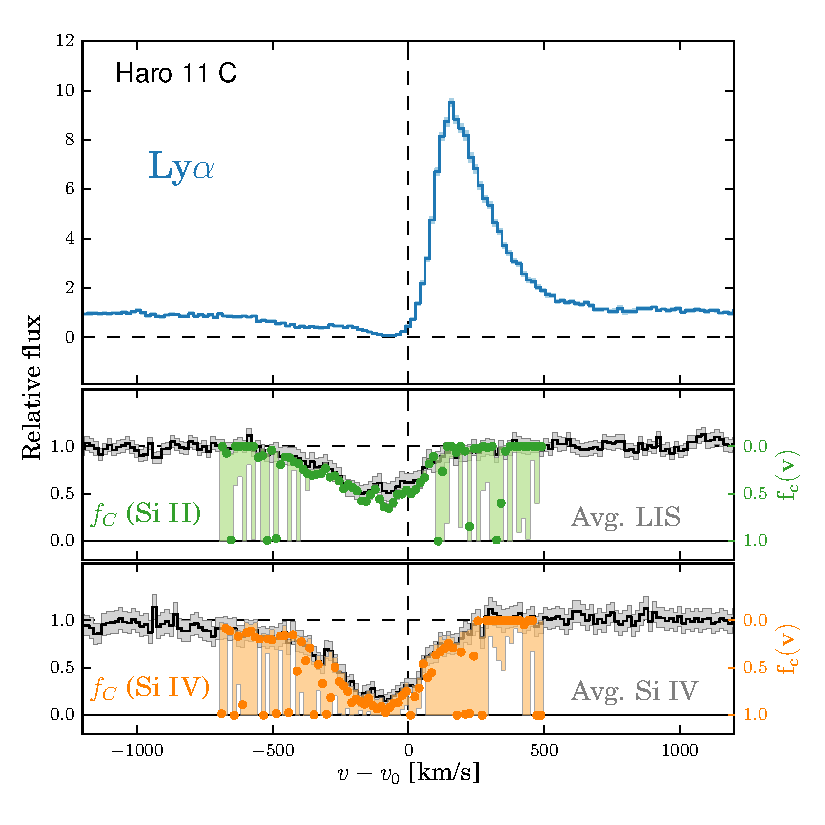
\includegraphics[width=3.500in]{../Figs/LyACoverfracs.pdf}
\caption{\textbf{Upper panel}: Ly$\alpha$ profile of Haro 11 C, in
approximate units of the surrounding continuum level. Full line is the
measured values smoothed by a 5 px. flat kernel; surrounding shading
encloses the $\pm 1 \sigma$ error band (mostly comparable in width to
the line width). \textbf{Middle panel}: Black steps show the averaged,
LIS line profile, smoothed by a 5px kernel. Surrounding gray shading
denotes the $\pm 1 \sigma$ confidence band. \textbf{Lower panel}: Same
as middle panel, but for the \ion{Si}{4} transitions.
}\label{fig:HisLisLya}
\end{figure}

The picture is what we would expect from a Lyman Continuum leaker: weak
neutral and strong ionized absorption profiles, the latter almost
everywhere consistent with full coverage, reveal a highly ionized medium
in front of the central cluster. This is also in good agreement with the
findings of \citet{Pardy2016arXiv}, who conclude that the galaxy has
about twice as much ionized as neutral gas. In addition to this, it is
interesting to note the close similarity in shape between the
\ion{Si}{2} and \ion{Si}{4} line profiles, indicating that they likely
represent two different phases in the same higher density regions. These
regions will likely be ionized on the side facing the central cluster,
being photoionized by its hot, massive stars. This also implies that the
nebular emission outflow found in {[}Rivera-Thorsen et al, submitted{]}
at least partially traces the same gas as the \ion{Si}{4} absorption
here and, by extension, also the neutral medium. Looking at
fig.~\ref{fig:SingleLines}, we see that maximum absorption and thus the
largest amount of gas in a single velocity bin for both phases is found
at around $v \approx -50$ km s⁻¹, where also a component is found in
{[}Rivera-Thorsen et al., submitted{]}. The outflow velocity
$v_{\text{int}}$ is at 149 ± 7 km s⁻¹, fully consistent with the
findings of \citet{Heckman2015} and \citet{Alexandroff2015}.
Interestingly, \citet{Sandberg2013} found from the neutral Sodium
resonance absorption doublet $\lambda \lambda 5889.95,5895.92$ (NaD) an
overall, weak \emph{redshift} of $v = 32$ km s⁻¹. From
e.g.~fig.~\ref{fig:HisLisLya}, it is evident that while neutral gas
\emph{is} present at these velocities, the velocity is at odds with the
integrated velocity of $v = -149$ km s⁻¹ found in this work. We note
that Na \textsc{i} has a very low ionization potential of only $\sim 5$
eV, meaning that these atoms may well only be present in the densest
and/or dustiest regions, in which Sodium is shielded from ionization.
This is in agreement with the finding of \citet{Sandberg2013} that NaD,
despite being a strong transition, shows absorption of only $\sim 95\%$
of continuum level and is mostly found in small, optically thick clouds.
This suggests that the NaD is tracing only the densest and/or dustiest
regions which are more slowly accelerated by star formation feedback
than the surrounding, more dilute medium. In fig.~\ref{fig:apert}, dusty
regions in the aperture are apparent E and W of knot C, and in the
better resolution of fig. 1 in \citet{Adamo2010}, these regions seem
like they might be connected by a narrow dust lane partially covering
the background source. We speculate that the NaD absorption of
\citet{Sandberg2013} might be associated with this.

Also the absorption feature in the Lyman $\alpha$ profile in the upper
panel seems to morphologically follow the shape of the metal lines,
indicating that radiative transfer effects are modest, indicative of a
fairly low column density of HI around line center. We find a Lyman
$\alpha$ peak velocity of $v_{\rm peak}^{\mathrm{Ly}\alpha} = 158 \pm 1$
km s⁻¹ w.r.t the systemic velocity found by \citet{Sandberg2013},
derived from nebular emission lines in the region around knot C. This
velocity, as it is also discussed in \citet{Verhamme2015}, is just
consistent with their theoretical predictions for a density-bounded,
low-column density system, albeit on the upper limit of their allowed
range.

\subsection{Metal and \ion{H}{1} column
density}\label{metal-and-column-density}

Lyman $\alpha$ escape is mainly governed by gas at or near systemic
velocity. In the middle panel of fig.~\ref{fig:WithColDens} (a) is shown
the best-fit column density $N_{\rm Si II}$ for each velocity bin. The
value at systemic velocity is $\log_{10}(N_{\rm Si II}) = 12.1 \pm 0.2$.
We adapt the value for local starbursts of log(Si/O) $= -1.59 \pm 0.07$
from \citet{Garnett1995}, and use this to estimate the column density of
neutral Hydrogen in front of the light source in the same way is in
{[}Puschnig et al., submitted to MNRAS{]} as follows. \citet{Guseva2012}
found a metallicity of Haro 11 C of $12 + \log_{10}(\text{O/H}) = 8.1$.
With $\log_{10}$ Si/O $= -1.59 \pm 0.07$, this leads to a Si/H ratio in
the neutral medium of Si / H $= 3.24^{+0.57}_{-0.48} 10^{-6}$, leading
to a Hydrogen column density of $6.2^{+0.9}_{-1.1} \times 10^{17}$
cm\textsuperscript{-2}. Since HI gets opaque to ionizing radiation at
$\log N \sim 17.2$ \citep{Verhamme2015}, this range is not consistent
with the low- optical depth, density bounded scenario. Furthermore;
while Ly$\alpha$ radiative transfer is dominated by gas of $v \sim v_0$,
Lyman continuum is sensitive to \ion{H}{1} at \emph{all} velocities.
Integrating the computed column densities over $-450$ km s⁻¹ $< v < 150$
km s⁻¹, the velocity range over which the column densities can be
reasonably well determined (and removing the unphysically high value in
the bin at $v \approx 222$ km s⁻¹), yields a conservative estimate of
$\log N_{\rm Si II} \approx 19.4$, corresponding to more than 150
optical depths in Lyman Continuum, strongly incompatible with an
optically thin, density-bounded scenario.

However, the pure riddled ionization bounded scenario is easily ruled
out since the Ly$\alpha$ profile does not have any appreciable emission
component at zero velocity. We therefore expect a residual neutral
fraction to remain in the ionized phase; a fraction which has a column
density high enough to block Ly$\alpha$ efficiently at line center, but
low enough to be at least part transparent to Lyman Continuum radiation
and undetected in \ion{Si}{2}.

We can estimate the lowest detectable $N_{\rm Si II}$ by noting that the
relative errors for the \ion{Si}{2} lines in our spectrum are
$\sim 0.05$. Assuming a covering fraction of unity for the dilute
neutral component, and adopting the oscillator strength of the strongest
of the \ion{Si}{2} transitions, $f\lambda_{1260 \AA} = 1486.8$, we find
in the limit that $I/I_0 = e^{-\tau} = 0.95$, and eq.~\ref{eq:tau}
becomes:
%
\begin{equation}
\label{eq:silim}
N_{\rm Si II}^{\rm min} = -\log_{e}(0.95) \frac{3.768 \times 10^{14}}{f\lambda} 
    = 10^{10.1} \text{cm}^{-2},
\end{equation}
%
 which with the adopted metallicity for Haro 11 C corresponds to a
minimum Hydrogen column density of
$N_{\rm HI}^{\rm min} \sim 4.0 \times 10^{15}$ cm⁻². This leaves around
2 orders of magnitude in $N_{\rm H I}$, in which the gas is not detected
in \ion{Si}{2} and is optically thick to Ly$\alpha$ while translucent to
Lyman Continuum. If we require the gas to be detected in at least two of
the lines included in this analysis, the limiting hydrogen column
density becomes $N_{\rm HI}^{\rm min} \sim 4.9 \times 10^{16}$ cm⁻²,
adding another order of magnitude to the allowed range, but we adopt the
lower value as a conservative estimate.

The existence of a diffuse neutral component being present in the
ionized medium seems consistent with what is found in the Green Pea
galaxies of \citep{Henry2015} - these galaxies have sometimes very low
LIS optical depth, which is usually indicative of low covering fractions
and high porosity of the neytral medium - and yet they find covering
fractions of near unity of \ion{H}{1} from Lyman $\beta$ absorption,
indicating column densities of $N \gtrsim 10^{16}$. Like in the case of
Haro 11, this indicates that a non-negligible neutral component must be
present in the ionized phase, although it may very well be of such low
densities and metallicity that metal absorption from this medium is
undetectable.

The column densities we derive for \ion{Si}{2} in this work are
generally between $12.0 \lesssim \log N \lesssim 12.5$, column densities
around which the transitions involved become optically thick: For
$\lambda \lambda 1260, 1526 \text{ and } 1304$, $\tau$ becomes 1 at
$\log N \sim 11.3, 12.2$ and $12.5$, respectively. Off the regions of
strongest absorption, and in particular at $v_0$, only $\lambda 1260$
seems to be optically thick, and it seems the column densities arrived
at can be trusted. But at line center, around $v\sim v_{int}$, the
column densities found are so close to the limit that they are most
likely to be interpreted as lower limits. There might also be
systematics in the determination of the continuum around the lines which
may lead to the lines at $\lambda \lambda 1304, 1526$ to be falsely seen
as shallower than $\lambda 1260$, meaning that all computed column
densities are really lower limits rather than actual values. The
confidence intervals in fig. \ref{fig:WithColDens} do \emph{not} reflect
this possible saturation, but only the formal errors from the best
approximation to the residual intensity, they do not include
systematics.

If the computed column densities are in fact lower limits, this means
the inferred \ion{H}{1} column densities are also lower limits. This
would strengthen the modified riddled, ionization-bounded medium
scenario that the ISM on the line of sight to Haro 11 C consists of
dense, neutral clumps with an ionized interclump medium containing a
dilute neutral component.

\subsection{Neutral gas metallicity}\label{neutral-gas-metallicity}

The exact value of the metallicity is however uncertain. The values
found from nebular recombination lines by \citet{Guseva2012} are
measured mainly in the central HII regions around the clusters; and
differ by 0.2 dex between knot B and C. The neutral, outflowing gas
could be mixed, or have an unseen LOS distance component larger than the
knot separation, drawing into question which is the better value to
assume for this gas. We base our conclusions on the value found for knot
C, but note that using the metallicity of $12 + \log (O/H) = 8.3$ found
for knot B by \citet{Guseva2012}, the inferred H \textsc{i} column
densities are $3.9 \pm 0.6 \times 10^{17}$ cm\textsuperscript{-2}.
However, the question of the exact metallicity of the outflowing gas is
complicated. Gas closer to the star forming regions is expected to be
more strongly enriched than gas further away, which would imply that the
HI column density is \emph{larger} than inferred from \ion{Si}{2} above.
To this can be added the further complication stemming from the merger
event that the galaxy is currently undergoing, which may have mixed gas
of different metal contents. In any case, though, we would expect the
regions nearest to the starbursts to generally have higher metallicity
than the surrounding cool gas, such that the HI column density inferred
above is more likely to be underestimated than overestimated.

\subsection{Radiative transfer effects}\label{sec:rt}

The conclusions drawn by the AOD method rest on the assumption that the
observed lines are close to being pure absorption lines, with
redistribution of photons due to radiative transfer effects being
modest. Modelling work by e.g. \citet{Prochaska2011} and
\citet{Scarlata2015} has shown that in certain conditions, radiative
transfer can re-fill absorption features in a way that can make an
isotropic, optically thin mimic the observational fingerprints of a
system of optically thick clumps. We therefore need to investigate
whether our conclusions could be generated by such effects.

\begin{figure}
\centering
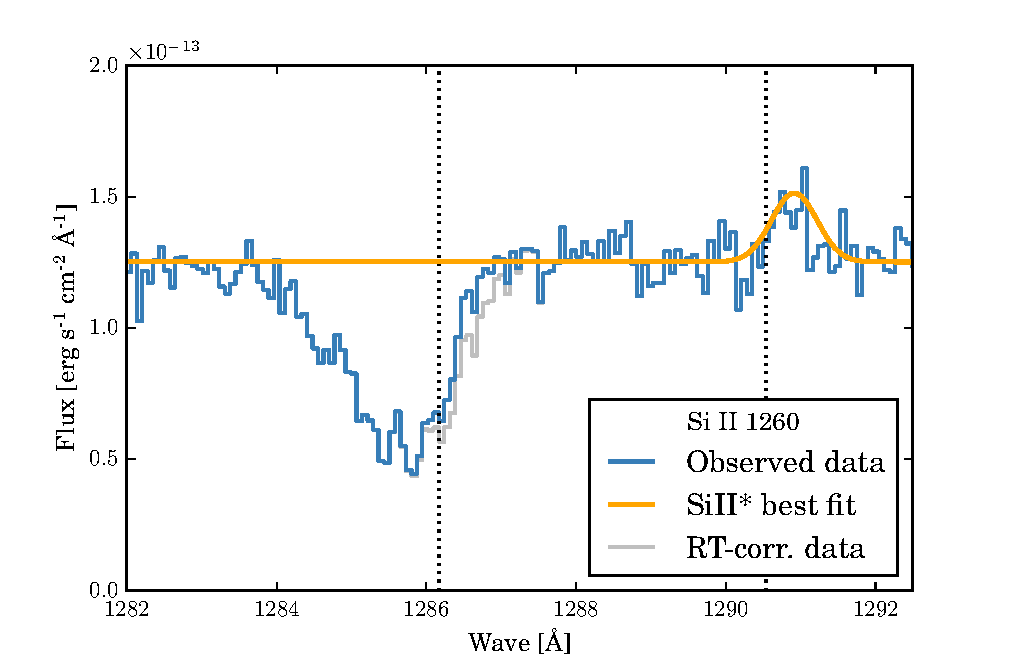
\includegraphics[width=3.500in]{../Figs/1260-fit-fluor.pdf}
\caption{\ion{Si}{2} $\lambda 1260$ and its fluorescent line at
$\lambda 1265$, with the observed data shown in blue. The orange curve
shows a fit to the fluorescent emission, and in gray is shown the
worst-case absorption profile corrected for radiative transfer effects
re-filling the absorption trough.}\label{fig:rt}
\end{figure}

Because the ground level in \ion{Si}{2} is a doublet with a short-lived
upper level, each of the Silicon lines included in the analysis has a
fluorescent emission line with practically no absorption component. The
fluorescent line can be used to constrain the possible effect of
radiative infilling of the absorption trough. If each photon in the
fluorescent transition on average has scattered once in the neutral
medium, the ratio of emission in this line and re-filling of the
resonant absorption line is simply that of their Einstein coefficients
$A_{ki}$. For each subsequent scattering, more photons escape directly
through the fluorescent channel, and the infilling of the absorption
line further suppressed.

In fig.~\ref{fig:rt}, the observed line profile is shown in blue, along
with the best fit to \ion{Si}{2}$^*$ shown in orange. Since the
fluorescent and resonant reemission originate in the same environments,
the shape of the resonant reemission profile can be completely
determined from the shape and center of the fluorescent line and the
assumption of one scattering. It is therefore simple to construct this
theoretical reemission line, subtract it from the observed absorption
line and find a lower limit for the depth of the pure absorption line
without reemission; this model line sis shown in gray in the figure. It
is readily seen that the difference between theoretical and observed
line is so small that it cannot affect our conclusions about the
covering factors and column densities of the neutral gas significantly.

We have not performed similar measurements for the lines at
$\lambda \lambda 1304, 1526$, but note that if significant refilling is
present here, this would mean the column densities had actually been
underestimated in our analysis, which would strengthen the conclusions
of a clumpy medium optically thick in \ion{Si}{2} $1260$, but part
transparent in the much weaker other lines.

\subsection{\ion{C}{2} $\lambda 1334$
absorption}\label{lambda-1334-absorption}

Looking back at Fig.~\ref{fig:SingleLines}, the profile of \ion{C}{2}
$\lambda 1334$ is clearly deeper than \ion{Si}{2} $\lambda 1260$, which
we had otherwise concluded is optically thick and thus provides a limit
for the velocity binned covering fractions. We believe the explanation
is a contribution from \ion{C}{2} $\lambda$ 1335.7 blending with
$\lambda 1334$. This transition has an oscillator strength of
$f_{ik} = 0.114$, compared to $f_{ik} = 0.127$ for $\lambda 1334$ (there
is a third line at 1335 Å, but that is an order of magnitude weaker), so
given a sufficient population of its ground level, it is strong enough
to make a non-negligible contribution to the resulting line profile. One
should however bear in mind that these lines rise from different lower
fine structure levels; $\lambda 1334$ arises from ²P$_{1/2}$, while the
other two arise from ²P$_{3/2}$. The population of the latter level
depends sensitively on physical conditions in its system of origin,
especially those in photo dissociation regions.

\begin{figure}
\centering
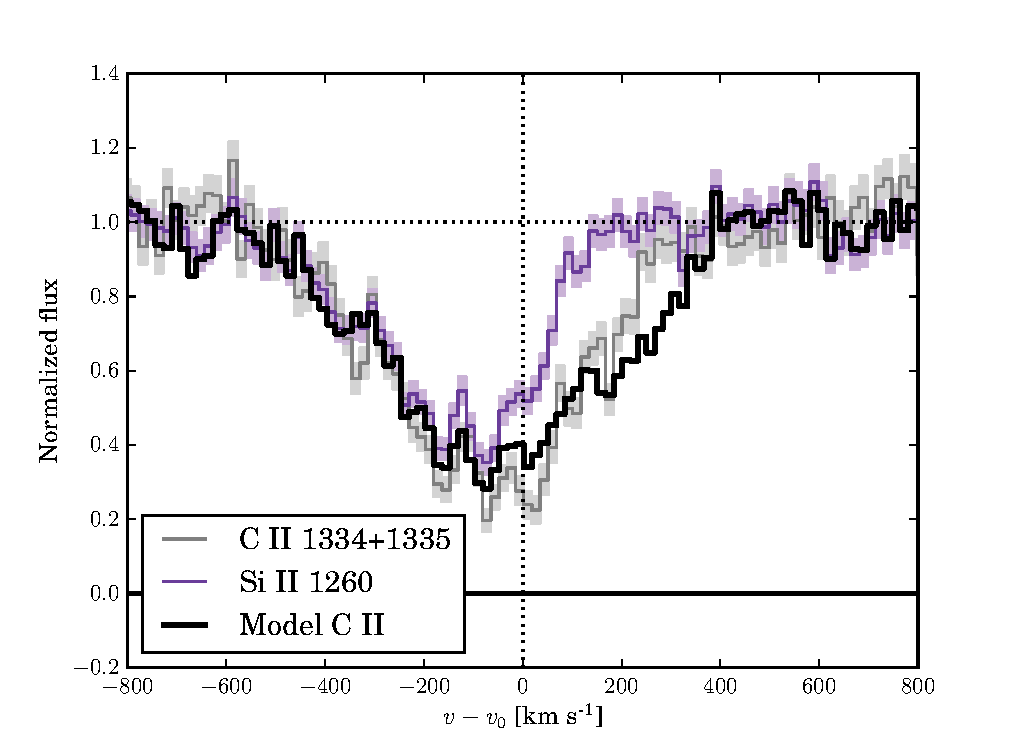
\includegraphics[width=3.500in]{../Figs/CIIdoubletmodel.pdf}
\caption{C \ion{C}{2} 1334, \ion{Si}{2} 1260, along with a \ion{C}{2}
line synthesized from \ion{Si}{2} (see text for
details).}\label{fig:CII}
\end{figure}

Fig.~\ref{fig:CII} shows a quick back-of-the-envelope check of this
hypothesis. Assuming the ions reside in the same physical regions, we
used the \ion{Si}{2} and a second contribution created by shifting the
original profile to the red by the appropriate velocity ($\sim 260$ km
s⁻¹) and multiplying it by a free parameter, which was chosen by eye to
give a reasonable replication of the observed \ion{C}{2}; the chosen
value shown in the figure is 0.7 times the original line. It is clear
from the figure that the reproduction of the observed \ion{C}{2} line is
very reasonable, considering that it is generated from a different
species with a very different ionization potential.

Whether this is a physically reasonable strength is difficult to say
with precision, but we note that to reproduce the feature observed,
$\lambda 1334$ must be optically thick and $\lambda 1335$ part
transparent. This leave open a degeneracy of relative level populations
and ion abundance, such that the choice of this value only weakly
constrains these quantities and thus it is compatible with a wide range
of scenarios.

It is also worth noting that \ion{C}{2} has a significantly higher
ionization potential than \ion{Si}{2}, such that the former will be more
abundant in regions of higher ionization, with \ion{C}{2} in effect
tracing slightly different regions than \ion{Si}{2}. Furthermore, in
these regions of higher ionization, the relative level populations of
the Carbon ground state can be significantly altered by shifts in
e.g.~electron density and radiation field, which can alter the line
shape further. We make no attempt at mapping these complex conditions
here, but note only that there exists a range of non-exotic physical
effects which can generate the deeper and wider $\lambda 1334$ profile
we observe while still being compatible with the ISM being optically
thick in \ion{Si}{2} $\lambda 1260$.

\subsection{Conclusion}\label{conclusion}

In this work, we have re-analyzed an archival FUV HST-COS spectrum to
investigate the kinematics and geometry of both the hot, ionized and
cold, neutral ISM along the LOS to the main star forming knot. We have
used the Apparent Optical Depth method to compute column densities and
velocity-binned covering fractions of the gas and compared these results
to the extreme cases of either an optically thin, density bounded
neutral medium, or a riddled, optically thick, ionization bounded
neutral medium. Assuming that the Lyman Continuum emission previously
observed from this galaxy indeed does originate from knot C, we find
that the observations are not compatible with the latter case, since the
characteristic, bright Lyman-$\alpha$ emission spike at line center is
absent in this spectrum. Furthermore, the observations are not
consistent with an optically thin, density bounded neutral medium.

We confirm previous authors concluding that the medium is highly ionized
with clumps of neutral gas of low velocity-binned covering fraction,
increasing the probability of finding direct sight lines to the
background star cluster between these. The clumps have HI column
densities of gas around $v=0$ in the range
$N_{\rm HI} = 6.2^{+0.9}_{-1.1} \times 10^{17}$ given the metallicity of
the background \ion{H}{2} region, which is likely a slight underestimate
of $N_{\rm HI}$. A conservative estimate of the \ion{H}{1} column
density integrated over all velocities is
$N_{\rm H I}^{\rm tot} \sim 2.5 \times 10^{19}$ cm⁻². There is a
possibility that the found column densities are in fact lower limits,
since the found \ion{Si}{2} column densities are close to the limit
where this ion becomes optically thick. We therefore conclude that the
leaked ionizing photons, if originating from this cluster, most likely
escaped via sight lines through the ionized medium, which must thus
contain a neutral gas column density
$5 \times 10^{13} \leq N_{\rm HI}^{\rm HIS} \leq 4 \times 10^{15}$. This
range is bounded downwards by the value at which HI becomes transparent
to Lyman-$\alpha$, and upwards by the sensitivity to \ion{Si}{2} of this
observation.

\section*{Acknowledgements}\label{acknowledgements}
\addcontentsline{toc}{section}{Acknowledgements}

GÖ \& MH acknowledge the support of the Swedish Research Council,
Vetenskapsrådet, and the Swedish National Space Board (SNSB) and M. H.
is an Academy Fellow of the Knut and Alice Wallenberg Foundation. This
project has made extensive use of the Python-based packages Numpy
\citep{Numpy}, SciPy \citep{SciPy}, Matplotlib \citep{Matplotlib},
Pandas \citep{Pandas}, LMfit \citep{lmfit2014}, and Astropy
\citep{Astropy2013}.

\bibliography{./main.bib}

\end{document}
